%
% LATEXBONES
%
\documentclass[a4paper,12pt,twoside]{article}
\usepackage{graphicx}
\usepackage{amsmath}
\usepackage[english]{babel}
\usepackage[applemac]{inputenc}
\usepackage[colorlinks,bookmarks=false,linkcolor=blue,urlcolor=blue]{hyperref}
\usepackage{subfigure}
\usepackage{here}
\usepackage{wrapfig}
\usepackage{fancyhdr}

%drow graph
\usepackage{fancybox}
\usepackage{tikz}
\usepackage{capt-of}
\usepackage{verbatim}


% print code
\usepackage{listings}
\usepackage{algorithm2e}

% landscape
\usepackage{pdflscape}

\paperheight=297mm
\paperwidth=210mm

\setlength{\textheight}{235mm}
\setlength{\topmargin}{-1.2cm} 

\setlength{\textwidth}{15cm}
\setlength{\oddsidemargin}{0.56cm}
\setlength{\evensidemargin}{0.56cm}

\pagestyle{plain}

\def \be {\begin{equation}}
\def \ee {\end{equation}}
%\def \dd  {{\rm d}}m


\newcommand{\mail}[1]{{\href{mailto:#1}{#1}}}
\newcommand{\ftplink}[1]{{\href{ftp://#1}{#1}}}

\def \ExprList {\textit{ExprList}}
\def \ClassList {\textit{ClassList}}
\def \ClassTree {\textit{ClassTree}}
\def \ScoreClassTree {\textit{ScoreClassTree}}
\def \DirectScoreTree {\textit{DirectScoreTree}}
\def \Completor {\textit{Completor}}

\def \pathExprList {\path{leon.comparison.ComparatorExprList}}
\def \pathClassList {\path{leon.comparison.ComparatorClassList}}
\def \pathClassTree {\path{leon.comparison.ComparatorClassTree}}
\def \pathScoreClassTree {\path{leon.comparison.ComparatorScoreClassTree}}
\def \pathDirectScoreTree {\path{leon.comparison.ComparatorDirectScoreTree}}
\def \pathCompletor {\path{leon.comparison.Completor}}



\fancyhead[L]{Applied Data Analysis}
\fancyhead[R]{Summary}



% ======= Document ======

\begin{document}
\begin{titlepage} %Titre
\begin{center}
\newcommand{\HRule}{\rule{\linewidth}{0.5mm}} % Defines a new command for the horizontal lines, change thickness here
\center % Center everything on the page
 
%----------------------------------------------------------------------------------------
% HEADING SECTIONS
%----------------------------------------------------------------------------------------



\begin{figure} [h] %----------- SubGraph ---------------------
\centerline{
\subfigure{\includegraphics[height = 2 cm]{pic/epfl}  }
\subfigure{\includegraphics[height = 2 cm]{pic/ada-logo}} 
} 
\end{figure}


\vspace{0.5cm}
%\textsc{\LARGE EPFL}\\[1.5cm] % Name of your university/college
\textsc{\Large School Of Computer And Communication Sciences}\\[0.5cm] % Major heading such as course name
\textsc{\Large }\\% Minor heading such as course title
%\textsc{ \Large Master Semester Project}\\ % Minor heading such as course title
%----------------------------------------------------------------------------------------
% TITLE SECTION
%----------------------------------------------------------------------------------------

\HRule \\[0.4cm]
{ \huge \bfseries Applied Data Analysis \\Summary}\\[0.4cm] % Title of your document
\HRule \\[1.5cm]

\begin{flushleft} \large
Prof. \textsc{Catasta} Michele\\
Distributed Information Systems Laboratory (LSIR) \\
\mail{michele.catasta@epfl.ch} \\ 
\end{flushleft}

 
%%----------------------------------------------------------------------------------------
%% AUTHOR SECTION
%%----------------------------------------------------------------------------------------

\begin{center}
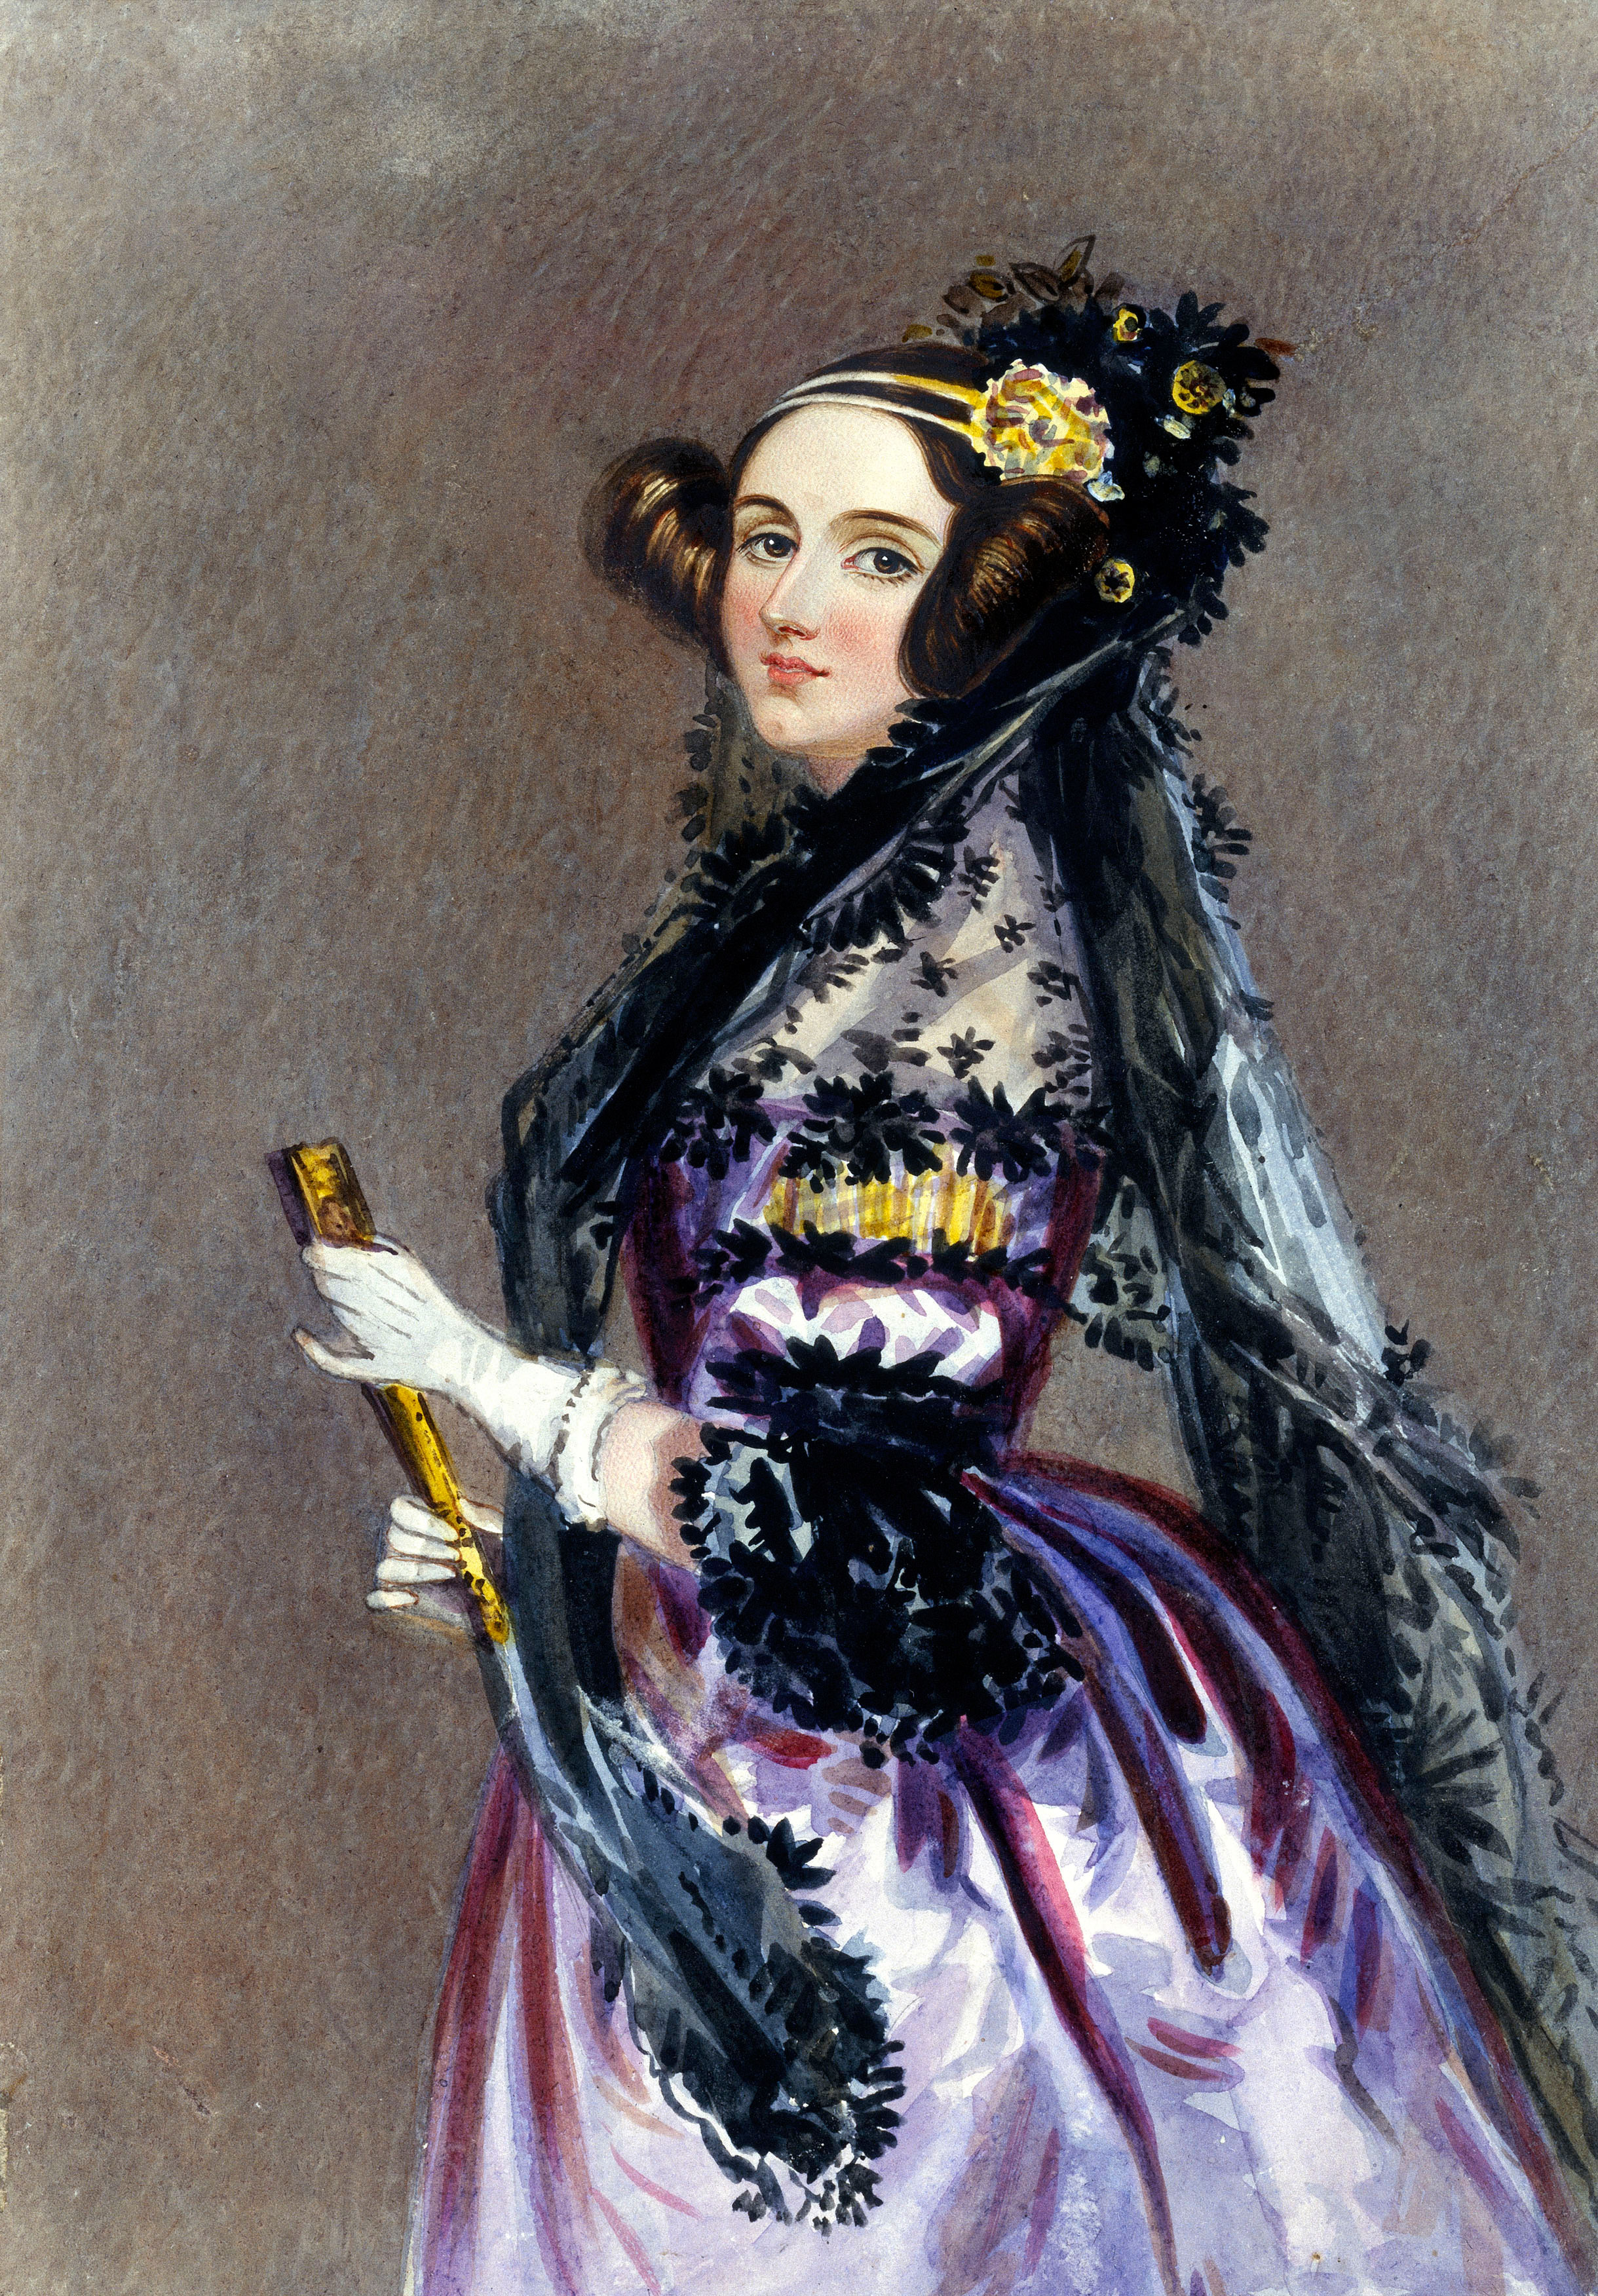
\includegraphics[width = 5 cm]{pic/lovelace} % Include a department/university logo - this will require the graphicx package
\end{center}
%
%
%
%
%
%\begin{minipage}[t]{0.4\textwidth}
%
%\end{minipage}
%~
%\begin{minipage}[t]{0.55\textwidth}
%%\begin{flushright} \large
%%\emph{Assistant:} \\
%%\textsc{Voirol} Nicolas \\
%%PhD student\\
%%\mail{nicolas.voirol@epfl.ch} \\ [0.4cm]
%%
%%\emph{Supervisor:} \\
%%\textsc{Kuncak} Viktor\\  % Supervisor's Name
%%Professor\\
%%LARA - Laboratory for Automated Reasoning and Analysis\\
%%\mail{viktor.kuncak@epfl.ch}
%%\end{flushright}
%\end{minipage}\\[2cm]

% If you don't want a supervisor, uncomment the two lines below and remove the section above
%\Large \emph{Author:}\\
%John \textsc{Smith}\\[3cm] % Your name

%----------------------------------------------------------------------------------------
% LOGO SECTION
%----------------------------------------------------------------------------------------



%----------------------------------------------------------------------------------------
% DATE SECTION
%----------------------------------------------------------------------------------------

%{\Large \today}\\[1cm] % Date, change the \today to a set date if you want to be precise

{\Large June 10, 2016}\\[1cm] % Date, change the \today to a set date if you want to be precise
%
%\begin{center}
%\abstract{\large Experiment various methods to compare functional trees between them. Given a function, use these algorithms to find the most similar tree contained in a corpus of functions. Try to suggest an autocompletion for a "hole" in a tree, based on this corpus.}
%\end{center} 
 %{\Large IDQ CONFIDENTIAL}
%----------------------------------------------------------------------------------------
\vfill % Fill the rest of the page with whitespace

\end{center}
\end{titlepage}



\pagestyle{fancy}
% ================Table des mati�res ==============
\newpage
\tableofcontents 

\baselineskip=16pt
\parindent=15pt
\parskip=5pt

\newpage




%=========================================
\section{Introduction} 


%======= TABLEAU ===========
%\begin{center} %---------------Tab--------------
%\begin{tabular} {| c | c | c | c | c | c |}
%\hline
 %& & & & & $\\ \hline
%\end{tabular}
%\end{center}


%===========GRAPH================
%\begin{figure} %---------------------Graph---------------------------
%\begin{center}
%\includegraphics[width=12cm]{graph/ampli2} 
%\end{center}
%\caption{\em  \label{label}
%L�gende
%}
%\end{figure}


%========SUBGRAPH=======
%\begin{figure} [h] %----------- SubGraph ---------------------
%\centerline{
%\subfigure[ sublegend ] {\label{sfig:thetat} \includegraphics[width=7cm]{ graph/graph_convdt3 } }
%\subfigure[ sublegend ] {\label{sfig:thetafin} \includegraphics[width=7cm]{ graph/graph_convtfin } } 
%}
%\caption{\label{ label } 
%L�gende
%} 
%\end{figure}








\end{document} %%%% THE END %%%%
